\documentclass[main.tex,fontsize=8pt,paper=a4,paper=portrait,DIV=calc,]{scrartcl}
% Document
\usepackage[T1]{fontenc}
\usepackage[dvipsnames]{xcolor}
\usepackage[nswissgerman,english]{babel}
\renewcommand{\familydefault}{\sfdefault}

% Format
\usepackage[top=5mm,bottom=1mm,left=5mm,right=5mm]{geometry}
%\setlength{\headheight}{\baselineskip}
%\setlength{\headsep}{0mm}

%\usepackage{scrlayer-scrpage}
%\clearpairofpagestyles
%\chead{{\bfseries\TITLE, \AUTHOR, \pagename~\thepage}}

%\addtokomafont{pagehead}{\upshape}

\usepackage{multicol}
\setlength{\columnsep}{2mm}
\setlength{\columnseprule}{0.1pt}

% Math
\usepackage{amsmath}
\usepackage{amssymb}
\usepackage{amsfonts}

% Code
\usepackage{fancyvrb, etoolbox, listings, xcolor}
%\usemintedstyle{bw}

%\newminted[shell]{bash}{
%fontsize=\footnotesize,
%fontfamily=tt,
%breaklines=true,
%frame=single,
%framerule=0.1pt,
%framesep=2mm,
%tabsize=2
%}
%\newminted{css}{
%breaklines=true,
%tabsize=4,
%autogobble=true,
%escapeinside=||,
%stripall=true,
%stripnl=true,
%}

    \definecolor{lightgray}{rgb}{0.95, 0.95, 0.95}
    \definecolor{darkgray}{rgb}{0.4, 0.4, 0.4}
    \definecolor{purple}{rgb}{0.65, 0.12, 0.82}
    \definecolor{ocherCode}{rgb}{1, 0.5, 0} % #FF7F00 -> rgb(239, 169, 0)
    \definecolor{blueCode}{rgb}{0, 0, 0.93} % #0000EE -> rgb(0, 0, 238)
    \definecolor{greenCode}{rgb}{0, 0.6, 0} % #009900 -> rgb(0, 153, 0)
    \definecolor{teal}{rgb}{0.0, 0.5, 0.5}

\lstdefinestyle{code}{
    identifierstyle=\color{black},
    keywordstyle=\color{blue}\bfseries\small,
    ndkeywordstyle=\color{greenCode}\bfseries\small,
    stringstyle=\color{ocherCode}\ttfamily\small,
    commentstyle=\color{teal}\ttfamily\textit\small,
    basicstyle=\ttfamily\small,
    breakatwhitespace=false,         
    breaklines=true,                 
    captionpos=b,                    
    keepspaces=true,                 
    showspaces=false,                
    showstringspaces=false,
    showtabs=false,                  
    tabsize=2,
    belowskip=-5pt
}



% Images
\usepackage{graphicx}
\newcommand{\pic}{\includegraphics[scale=0.3]}
\graphicspath{{Screenshots/}{../Screenshots}}
\makeatletter
\def\pictext#1#2{%
    \@ifnextchar[{%
    \pictext@iiiii{#1}{#2}%
    }{%
      \pictext@iiiii{#1}{#2}[0.5,0.4,0.3]% Default is 5
    }%
}
\def\pictext@iiiii#1#2[#3,#4,#5]{\begin{minipage}{#3\textwidth}\includegraphics[scale=#4]{#1}\end{minipage}\begin{minipage}{#5\textwidth}#2\end{minipage}}
\def\minipg#1#2{%
    \@ifnextchar[{%
    \minipg@iiii{#1}{#2}%
    }{%
      \minipg@iiii{#1}{#2}[0.3,0.6]% Default is 5
    }%
}
\def\minipg@iiii#1#2[#3,#4]{\vspace{0.8mm}\begin{minipage}{#3\textwidth}#1\end{minipage}\begin{minipage}{#4\textwidth}#2\end{minipage}{\vspace{0.8mm}}}
\makeatother

%\newenvironment{minty}[2]% environment name
%{% begin code
%  \begin{minipage}{#1}
%  \begin{minted}{#2}
%}%
%{% end code
%  \end{minted}
%  \end{minipage}
%  \end{minty}\ignorespacesafterend
%} 

% Smaller Lists
\usepackage{enumitem}
\setlist[itemize,enumerate]{leftmargin=3mm, labelindent=0mm, labelwidth=1mm, labelsep=1mm, nosep}
\setlist[description]{leftmargin=0mm, nosep}
\setlength{\parindent}{0cm}

% Smaller Titles
\usepackage[explicit]{titlesec}

%% Color Boxes
\newcommand{\sectioncolor}[1]{\colorbox{black!60}{\parbox{0.989\linewidth}{\color{white}#1}}}
\newcommand{\subsectioncolor}[1]{\colorbox{black!50}{\parbox{0.989\linewidth}{\color{white}#1}}}
\newcommand{\subsubsectioncolor}[1]{\colorbox{black!40}{\parbox{0.989\linewidth}{\color{white}#1}}}
\newcommand{\paragraphcolor}[1]{\colorbox{black!30}{\parbox{0.989\linewidth}{\color{white}#1}}}
\newcommand{\subparagraphcolor}[1]{\colorbox{black!20}{\parbox{0.989\linewidth}{\color{white}#1}}}

%% Title Format
\titleformat{\section}{\vspace{0.5mm}\bfseries}{}{0mm}{\sectioncolor{\thesection~#1}}[{\vspace{0.5mm}}]
\titleformat{\subsection}{\vspace{0.5mm}\bfseries}{}{0mm}{\subsectioncolor{\thesubsection~#1}}[{\vspace{0.5mm}}]
\titleformat{\subsubsection}{\vspace{0.5mm}\bfseries}{}{0mm}{\subsubsectioncolor{\thesubsubsection~#1}}[{\vspace{0.5mm}}]
\titleformat{\paragraph}{\vspace{0.5mm}\bfseries}{}{0mm}{\paragraphcolor{\theparagraph~#1}}[{\vspace{0.5mm}}]
\titleformat{\subparagraph}{\vspace{0.5mm}\bfseries}{}{0mm}{\subparagraphcolor{\thesubparagraph~#1}}[{\vspace{0.5mm}}]

%% Title Spacing
\titlespacing{\section}{0mm}{0mm}{0mm}
\titlespacing{\subsection}{0mm}{0mm}{0mm}
\titlespacing{\subsubsection}{0mm}{0mm}{0mm}
\titlespacing{\paragraph}{0mm}{0mm}{0mm}
\titlespacing{\subparagraph}{0mm}{0mm}{0mm}

%% format cells
\usepackage[document]{ragged2e}
\usepackage{array, makecell}
\renewcommand{\arraystretch}{2}
\newcommand{\mc}{\makecell[{{m{1\linewidth}}}]}


%%%%%define html as viable language
\lstdefinelanguage{CSS}{
    sensitive=true,
    keywords={%
    % JavaScript
    typeof, new, true, false, catch, function, return, null, catch, switch, var, if, in, while, do, else, case, break,
    % HTML
    html, title, meta, style, head, body, script, canvas,
    % CSS
    color:, border-radius:, border:, transform:, -moz-transform:, transition-duration:, transition-property:,
    transition-timing-function, background:, background-size:, background-color:, background-image:, background-origin:, background-repeat:, background-position:, background-attachement:, border:, border-box:, border-width:, border-color:, border-bottom:, border-style:, border-radius:, border-spacing:, border-collapse:, text-transform:, text-decoration-thickness:, text-align:, text-indent:, text-shadow:, text-justify:, text-overflow:, text-decoration:, text-align-last:, text-decoration-line:, text-decoration-color:, text-decoration-style:, margin:, padding:, 
    },
    % http://texblog.org/tag/otherkeywords/
    otherkeywords={<, >},   
    ndkeywords={class, export, boolean, throw, implements, import, this},   
    comment=[s]{/*}{*/},
    morecomment=[l]//,
    morecomment=[s]{<!}{>},
    morestring=[b]',
    morestring=[b]",    
    alsoletter={-},
    alsodigit={:}
}
\lstset{
    language=CSS,
    style=code,
}
%%%%%

\begin{document}
\begin{table}[h!]
\section{CSS}
\subsection{Syntax}
\begin{tabular}{|m{0.35\linewidth}|m{0.605\linewidth}|}

\hline
%\begin{csscode}
\begin{lstlisting}
body { 
    color: red;
}
\end{lstlisting}
%\end{csscode}
&
The first part is the element you want to modify, this can be the body, header, footer, a class like .button or even everything like with *. You can also add them together like: body, header, .button. \newline
\textbf{All selectors: \#id .class element.class * element element[ attribute ]}\\

\hline
\begin{lstlisting}
/*inline css*/
<p style="color:red;">
    This is a paragraph.
</p>
\end{lstlisting}
&
You can also use css right inside html if you for some reason want to do this. But please only do this when you have a single thing that needs something simple like a color. \newline For everything else use stylesheets.
\\

\hline
\begin{lstlisting}
/*full css inside html*/
<style>
body {
  background-color: linen;
}
</style>
\end{lstlisting}
&
You can of course also use a stylesheet inside html, also pretty useless, just use a proper stylesheet.
\\

\hline
\begin{lstlisting}
/*This is a comment*/ 
/*This is a 
multiline comment*/
// This is also a comment
\end{lstlisting}
&
The comments are made with these /* */ or //. Multilines are also allowed.
\\
\hline
\begin{lstlisting}
color: value|initial|inherit;
\end{lstlisting}
&
Besides the actual values, you can always use initial for the default values, or inherit for the value of the parent.\\
\hline
\begin{lstlisting}
p {
color: red;
}

div {
color: blue;
}

div p {
color: green;
}
\end{lstlisting} &
\textcolor{red}{\textbf{\emph{specifity:}}} \newline
If you have 2 rules that affect 1 element. For example color red and blue, then the most specific rule will win.\newline
For example, consider a paragraph inside a div.\newline
In this case div p is the most specific rule, then followed by p and div.\newline
Aka order: \textcolor{green}{green} \textcolor{red}{red} \textcolor{blue}{blue}\\
\hline
\begin{lstlisting}
h1 {
font-weight: bold;
font-size: 20px; !important;
}
h1 {
font-size: 30px;
}
\end{lstlisting}
& You can override rules with \textbf{\textcolor{red}{!important}} if you specifically want a lower case rule to take effect instead!\newline
\textcolor{red}{Should always be avoided if you can!}\\
\hline
\begin{lstlisting}
<link rel="stylesheet" href="style.css">
<link rel="stylesheet" href="https://shitgaem.online">
\end{lstlisting} & 
Proper link styles can be inserted with <link>. You can also embed a stylesheet from the internet!\\
\hline
\begin{lstlisting}
tr.warning td:nth-child(1)::before{
  color: red;
  content: "\26A0";
}
\end{lstlisting}
& This selects the td of a tr in class warning. Then goes to the nth-child, here 1 and before the content of said td.\newline
Then you can add new content with content: "something";\newline
Keep in mind that any changes with color etc are only made to this new content,\newline 
as you specify it above!
\\
\hline
\begin{lstlisting}
some-element::before {
  display: none;Glace
}
\end{lstlisting}
& If you would like to not display something from the html files, you can do this by specifying
display none before the content in question. \newline Keep in mind that this does not remove the content altogether, it only hides it!
\\
\hline
Inheritance & 
Inheritance in css is only applied sparsely, the reason for this is that you can still overwrite it with pretty much any selector, no matter how low the specificity is.\newline
\textcolor{orange}{If you want something to use inheritance then you need to explicitly state this!}\\
\hline
\end{tabular}
\begin{tabular}{|m{0.977\linewidth}|}
\hline
\textbf{Important note for CSS. If you want to affect an elements position, you will always have to change the attributes in the parent. \newline
In other words, justify-content and similar need to be defined in the box parent, not the div that you want to center!}\\
\hline
\end{tabular}
\end{table}
\pagebreak
\begin{table}[h!]
\subsection{Colors}
\begin{tabular}{|m{0.205\linewidth}|m{0.75\linewidth}|}

\hline
\begin{lstlisting}
color: red;
/* or */
color: #55667788;
/* #RRGGBBAA */
\end{lstlisting}
&
Colors are straight forward, you can either write the name of preconfigured colors, or use the RBGA values. \newline A is opacity.
\\

\hline
\end{tabular}
\subsection{Background}
\begin{tabular}{|m{0.975\linewidth}|}
\hline
\begin{lstlisting}
background-color: red;
background-image: "/path"; /* can also be an url -> url(https://...)*/
background-size: cover|auto|length|percentage|contain;
// cover: resizes to parent, auto: size of image, contain: resize image to fit inside parent, initial: fixed x,y value
background-position: x-value y-value; // top right, top center, center center, ...   Can also be x% y% default 0% 0%.
background-attachement: scroll|fixed|local; // local: scrolls with element, scroll is default.
// this decides if the background scrolls with the page or not.
background-origin: padding-box|content-box|border-box; 
// Used to define where the background image starts inside a box, only works when background-attachement is not fixed.
background-repeat: repeat|repeat-x|repeat-y|no-repeat|space|round; //useless shit
\end{lstlisting}
\\

\hline
\end{tabular}
\subsection{Borders}
\begin{tabular}{|m{0.975\linewidth}|}
\hline
\begin{lstlisting}
border: 4px solid red;
border: border-width border-style border-color;
border-style: none|hidden|dotted|dashed|solid|double|groove|ridge|inset|outset|initial|inherit;
//styles like ridge, groove, inset and outset use 3D effects, hard to describe.
border-radius: 4px 4px 4px 4px; // border-radius: 5px; also possible
//borders can be addressed individually by specifying a direction:
border-bottom: 4px solid red;
border-collapse: separate|collapse|initial|inherit;
// collapse means borders will merge in boxes. seperate will draw borders for both elements.
border-spacing: 4px; //Spacing between borders if the border-collapse is enabled!
\end{lstlisting}\\
\hline
\end{tabular}
\subsection{Margins and Paddings}
\begin{tabular}{|m{0.355\linewidth}|m{0.6\linewidth}|}
\hline
\begin{lstlisting}
margin: top right bottom left;
margin: 10px 10px 10px 10px;
padding: top right bottom left;
padding: top right bottom left;
//margin-right padding-left etc work as well.
\end{lstlisting}
&
Margin is the spacing between the element itself and it's parent and or other elements in the same hierarchy.\newline
Padding is the spacing inside the element to the contents of said element.
\\

\hline
\end{tabular}
\end{table}
\pagebreak
\begin{table}[h!]
\subsection{Text}
\begin{tabular}{|m{0.975\linewidth}|}
\hline
\begin{lstlisting}
text-align: left|right|center|justify; // justify is text as a block.
text-align-last: left|right|center|justify; //The last line can be configured indiidually.
text-justify: auto|inter-word|inter-character|none; /* only used when text-align is set to justify.
inter-word increases spacing between words, inter-character for characters.*/
text-decoration: text-decoration-line text-decoration-color text-decoration-style text-decoration-thickness;
text-decoration-line: none|underline|overline|line-through;
text-decoration-style: solid|double|dotted|dashed|wavy;
text-decoration-thickness: auto|from-font|value;
text-indent: value;
text-overflow: clip|ellipsis|string; 
//clip will just cut the string off, ellipsis ends with ..., a string will display itself.
text-shadow: h-shadow v-shadow blur-radius color|none;
text-transform: none|capitalize|uppercase|lowercase;
\end{lstlisting}
\\
\hline
\end{tabular}
\end{table}
\pagebreak
\begin{table}[h!]
\subsubsection{Fonts}
\begin{tabular}{|m{0.975\linewidth}|}
\hline
\begin{lstlisting}
font: font-style font-variant font-weight font-size/line-height font-family
|caption|icon|menu|message-box|small-caption|status-bar; //use the font used by this element
font-style: normal|italic|oblique; //oblique seems to be the same as italic.
font-variant: normal|small-caps;
font-weight: normal|bold|bolder|lighter|number; //number in 100 steps -> 100,200,300,...,900
font-size: medium|xx-small|x-small|small|large|x-large|xx-large|smaller|larger|length;
line-height: normal|number|length;
font-family: family-name|generic-family; //generic-family example: Isoveka
\end{lstlisting}
\\

\hline
\end{tabular}
\subsection{Display, justify and align}
\begin{tabular}{|m{0.975\linewidth}|}
\hline
\begin{lstlisting}
display: none|inline|block|contents|flex|grid|inline-block|inline-flex|inline-grid|inline-table|list-item|run-in|table|
         table-caption|table-column-group|table-footer-group|table-row-group|table-cell|table-column|table-row;
\end{lstlisting}\\
\hline
\end{tabular}
\subsection{Selectors and Combinators}
\begin{tabular}{|m{0.3\linewidth}|m{0.655\linewidth}|}
\hline
\textbf{Selectors}\newline
\begin{lstlisting}
selector::pseudo-element {
property: value;
}
\end{lstlisting}
& Pseudo selectors can be used to select only a specific part of an element.\newline
\pic{2022-10-04-10:58:46.png}\\
\hline
\textbf{Combinators and selectors} & 
\minipg{\pic{2022-10-04-11:03:12.png}}{\pic{2022-10-04-11:03:26.png}}[0.35,0.5]\\
\hline
\begin{lstlisting}
:is (box, button, something) p:hover {
background-color: red;
something-else: value;
}
\end{lstlisting}
& This applies a rule to all button box and something elements if hovered.\\
\hline
\begin{lstlisting}

\end{lstlisting}\\
\hline
\end{tabular}
\section{boxes}
\begin{tabular}{|m{0.3\linewidth}|m{0.655\linewidth}|}
\hline
\textbf{\emph{content-box and border box}} & \minipg{
  \textbf{content-box} increases the box size to ensure the child \textbf{element has the set size}.\newline
  \textbf{border-box} decreases the element size to ensure \textbf{the box itself has the set size}.
}{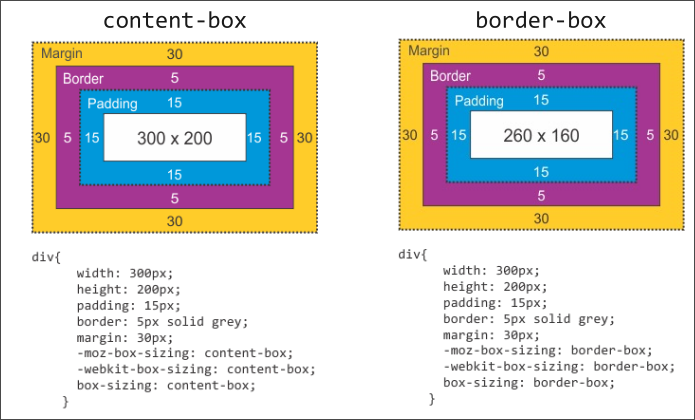
\includegraphics[scale=0.3]{2022-10-04-11:35:35.png}}[0.3,0.5]\\
\hline
\end{tabular}
\end{table}
\begin{table}[h!]
\begin{tabular}{|m{0,205\linewidth}|m{0.75\linewidth}|}
\hline
\mc{}\\
\hline
\end{tabular}
\end{table}
\begin{table}[h!]
\begin{tabular}{|m{0,205\linewidth}|m{0.75\linewidth}|}
\hline
\mc{}\\
\hline
\end{tabular}
\end{table}
\begin{table}[h!]
\begin{tabular}{|m{0,205\linewidth}|m{0.75\linewidth}|}
\hline
\mc{}\\
\hline
\mc{display: flex} & \mc{dynamically allocates spaces for elements inside this element.
usually combined with justify-content to adjust element position.} \\
\hline
\mc{min-height and min-width} & \mc{This should be used instead of width and height because an object might grow bigger than the max size. This will eventually break the look of the page, or break the application -> see eww.} \\
\hline
\end{tabular}
\end{table}
\end{document}

